\section{Introduction}
\label{motivation_engagement_introduction}
In this chapter we will discuss the concept of motivation and how it can be used to describe the interactions that individuals have with particular objects or activities. We will first provide a general introduction to the construct of motivation followed by a short historical review of theories of reward-driven motivation. We will then focus on how these led to the incentive salience hypothesis formulated by Berridge and Robinson \cite{berridge1998role}. While acknowledging the contribution of other theories in the definition of motivation (and reward-driven motivation in particular) this thesis will mostly focus on the areas of behavioural and affective neuroscience and make use of the framework provided by Berridge and Robinson \cite{berridge1998role}. The reason behind this choice lies in the fact that we found incentive salience to be more specific to motivation and most importantly to have a more robust and clear connection to behaviour. \lorem
The chapter closes with an overview on the idea that latent states, like those generated by incentive salience, might be represented as a manifold embedded in patterns of brain activity and behaviour.

\section{Motivation as a Reward-Driven Process}
\label{motivation}
The construct of motivation is a key concept for understanding why individuals seek out specific objects or experiences at particular times and why they react in particular ways when encountering objects considered of particular relevance \cite{berridge2004motivation}. In this view motivation can be defined as the process leading to the modulation and reiteration of goal directed behaviours that once reached exerts positive effects on the individual \cite{simpson2016behavioral}. A formal definition of motivation should encompass both the behavioural and the underlying psychobiological level. We will focus first on behavioural aspects of the process and outline in the following sections a theoretical account of motivation which also covers the psychobiological level. As we mentioned before, motivation describes why individuals react in particular ways when encountering objects regarded of high relevance and why they approach those objects at particular times \cite{berridge2004motivation}. These type of objects are said to possess "rewarding properties", which can be defined as the positive value ascribed to an object, a behavioral act or an internal physical state as the result of an active process of the mind and the brain \cite{schultz1997neural,berridge2008affective}. Importantly, motivation is not just driven by the fulfilment of fundamental needs like nutrition or reproduction (so-called "primary reward objects" \cite{schultz2000reward}) or the avoidance of negative consequences like physical pain. It also extends to those volitional objects and activities which do not appear to be necessary for the survival of the individual (i.e. "secondary reward objects" \cite{berridge2008affective,sescousse2013processing}). For those activities the expectation of the amount of reward received is learned over time and may vary significantly between individuals \cite{berridge2008affective,simpson2016behavioral}.In spite of this, it would be inefficient to have dedicated and specialized motivational systems for every combination of individuals and objects (e.g. an individual's motivation for playing sport or eating food). Instead, we can think of motivation as a single overarching entity that controls the interaction between individuals and objects in an agnostic manner \cite{simpson2016behavioral}. An analogy may be drawn with the geometric concept of a vector. Looking at Figure \ref{fig: vect_mot} we can imagine the focus on a specific object being represented by the angle of the vector while its length is the intensity of the motivational process (or the amount of motivated behaviour) \cite{simpson2016behavioral}. This, can be thought as a dynamic quantity defined by the state of the individual and the rewarding properties of the object \cite{toates1994comparing,berridge2004motivation,zhang2009neural}.
\begin{figure}[h]
  \begin{center}
    \begin{adjustbox}{width=0.5\columnwidth}
        \tikzset{every picture/.style={line width=0.75pt}} %set default line width to 0.75pt        
            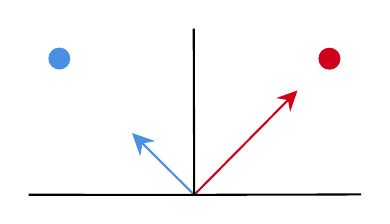
\begin{tikzpicture}[x=0.75pt,y=0.75pt,yscale=-1,xscale=1]
            %uncomment if require: \path (0,300); %set diagram left start at 0, and has height of 300
            
            %Straight Lines [id:da17586827840068286] 
            \draw [color={rgb, 255:red, 208; green, 2; blue, 27 }  ,draw opacity=1 ]   (190.24,200.32) -- (237.89,152.16) ;
            \draw [shift={(240,150.03)}, rotate = 494.69] [fill={rgb, 255:red, 208; green, 2; blue, 27 }  ,fill opacity=1 ][line width=0.08]  [draw opacity=0] (9.82,-4.72) -- (0,0) -- (9.82,4.72) -- (6.52,0) -- cycle    ;
            %Straight Lines [id:da23704064540856618] 
            \draw [color={rgb, 255:red, 74; green, 144; blue, 226 }  ,draw opacity=1 ]   (190.24,200.32) -- (162.38,172.64) ;
            \draw [shift={(160.25,170.53)}, rotate = 404.81] [fill={rgb, 255:red, 74; green, 144; blue, 226 }  ,fill opacity=1 ][line width=0.08]  [draw opacity=0] (10.72,-5.15) -- (0,0) -- (10.72,5.15) -- (7.12,0) -- cycle    ;
            %Shape: Circle [id:dp3839733612485111] 
            \draw  [color={rgb, 255:red, 208; green, 2; blue, 27 }  ,draw opacity=1 ][fill={rgb, 255:red, 208; green, 2; blue, 27 }  ,fill opacity=1 ] (250.58,134.73) .. controls (250.58,132.08) and (252.73,129.93) .. (255.38,129.93) .. controls (258.03,129.93) and (260.18,132.08) .. (260.18,134.73) .. controls (260.18,137.38) and (258.03,139.53) .. (255.38,139.53) .. controls (252.73,139.53) and (250.58,137.38) .. (250.58,134.73) -- cycle ;
            %Shape: Circle [id:dp009447430116501954] 
            \draw  [color={rgb, 255:red, 74; green, 144; blue, 226 }  ,draw opacity=1 ][fill={rgb, 255:red, 74; green, 144; blue, 226 }  ,fill opacity=1 ] (120.47,134.66) .. controls (120.47,132.02) and (122.61,129.88) .. (125.25,129.88) .. controls (127.89,129.88) and (130.03,132.02) .. (130.03,134.66) .. controls (130.03,137.29) and (127.89,139.43) .. (125.25,139.43) .. controls (122.61,139.43) and (120.47,137.29) .. (120.47,134.66) -- cycle ;
            %Straight Lines [id:da5714219654763008] 
            \draw    (190,120.28) -- (190.24,200.32) ;
            %Straight Lines [id:da22247567054966455] 
            \draw    (110.5,200.28) -- (190.24,200.32) ;
            %Straight Lines [id:da4124676757039665] 
            \draw    (270.64,200.12) -- (190.24,200.32) ;
            
            
            
            
            \end{tikzpicture}
    \end{adjustbox}
  \end{center}
\caption{\textbf{Motivation as a vector}. Blue and red dots represent two objects with different characteristics while the two arrows illustrate the hypothetical motivational propensity of an individual (or two individuals) towards them. The black segments delineate the space created by the combination of the objects' characteristics and the motivational propensity of the individuals. Here the red object has the potential to generate more behaviour than the blue object possibly as a result of its characteristics and those of the individual interacting with it.}
\label{fig: vect_mot}
\end{figure}
Summarizing we can say that from a motivational point of view, the behaviour of an individual is driven by the expectancy of pleasurable outcomes derived by the goal the behaviour is aiming to reach \cite{berridge2004motivation}. Therefore, if motivation acts as a single overarching process, we expect it to hold predictive and explanatory power over goal directed behaviour seamlessly across a heterogeneous range of situations and individuals. Motivational theories based on the concepts of reward and incentive are promising candidates for this because, relying on consistent and plausible psychobiological bases, they tend to operate abstracting from the nature of the individuals and the objects. \cite{ikemoto1999role,berridge1998role,salamone2002motivational,berridge2004motivation,armony2013cambridge,corbit2015learning}.

\subsection{An Historical View on Reward-driven Motivation}
\label{motivation_hist}
Introducing the processes of classical and operant conditioning is an essential step for describing theories of reward-driven motivation, in particular if we are interested in their behavioural correlates. Both constructs heavily rely on the general concepts of reinforcer and reinforcement process. Simply put, reinforcers are those objects or actions that have the ability to alter the likelyhood of appearance of specific behaviours \cite{kling1971woodworth,skinner1953science,squire2012fundamental}. A reinforcement process instead define the learning mechanisms by which a specific behaviour becomes, over time, more or less probable conditional on the presence of particular reinforcers \cite{kling1971woodworth}. In this view we can think of classical and operant conditioning as two complementary oprationalizations of the reinforcement process. Classical conditioning describes the learning process in which, independently from the activity of an individual, the repeated pairing of two objects will cause one to acquire the eliciting properties of the other \cite{squire2012fundamental}. In other words, the repeated pairing of a neutral object with reinforcing consequences will imbue the first with reinforcement properties making it a reinforcer. Operant conditioning on the other hand, extends the concept of classical conditioning introducing the agency of the individual \cite{skinner1953science}. The frequency of behaviour produced by an individual tends to increase when precise consequences are associated to it \cite{skinner1953science}. In this view, an operant is formalized as a goal directed behaviour while all the elements reinforcing the re-iteration of this behaviour are called reinforcers \cite{skinner1953science}. The learning process here results from the relationship between a behaviour and its consequences, therefore the probability of behaviour to take place is related to its capability to generate reinforcer \cite{kling1971woodworth}. Both classical and operant conditioning are of course very simplistic accounts of human behaviour, but nevertheless able to succinctly illustrate a fundamental process by which most (if not all) individuals are able to learn and leverage the association between actions and the positive (i.e. rewarding) consequences associated to them. In this regard, it is not surprising that many theories of reward-driven motivation stem directly from these two constructs. For example, in its work Bolles \cite{bolles1972reinforcement} suggested that individuals were motivated by the "expectations of incentive outcomes". These expectations are formed through a learning process where an association between actions and potential pleasurable outcomes is created \cite{bolles1972reinforcement,berridge2004motivation}. Expanding on this idea, Bindra suggested that the learning process does not just generate pleasure expectations in response to specific behaviours but it also allows individuals to perceive the behaviours themselves as a source of hedonic reward \cite{bindra1978adaptive,berridge2004motivation}.
This introduces the concept of learning through reinforcement: an object and the behaviours associated to it become relevant and salient for an individual as a consequence of learning its incentive properties \cite{berridge2004motivation}. A third theoretical formulation by Toates \cite{toates1994comparing}, asserted that the magnitude of the perceived incentives introduced by both Bolles and Bindra is modulated by the internal states of the individual \cite{toates1994comparing,berridge2004motivation}. In other words, the incentive expectations (and consequently the associated motivated behaviours) learned by an individual can change over time depending on the individual's internal state. Until now we have mainly used the terms reinforces and incentives for identifying objects able to drive and shape behaviour, but when it comes to define effective reinforces, it is not just a matter of merely pairing a behaviour with a stimulus but the stimulus itself has to have particular properties. In this view, stimuli able to generate pleasurable feelings in the individual are the best candidates for being effective reinforces, they are said having ‘rewarding properties’. But what is, and how can be defined the reward? The reward is a process generated in response to a stimulus making it desirable for its capacity to generate pleasurable responses. In this view, for being able to generate rewarding response, a stimulus needs two fundamental properties: it has to be wanted (i.e. it acquires the capacity to become desirable) and liked (i.e. it has to be able to generate pleasure in the individual) \cite{berridge2009dissecting}. But how a particular object acquires these properties? This is mostly carried out by the same learning processes mentioned in section \ref{motivation_hist}. The repeated pairing of a stimulus with the (positive) consequences it exerts on the individual will imbue the first with so called rewarding properties. Moreover, through operant conditioning  not just the stimulus itself but also the connected instrumental behaviour will likely acquire the same rewarding properties \cite{berridge2009dissecting}. As anticipated in section \ref{motivation}, a useful distinction that can be made is between objects having primary and secondary reward properties. Objects linked with essential evolutionary needs (i.e. satisfaction of homeostatic needs) are on a fast track for becoming reinforcers, their rewarding properties don’t have to be learned but are, up to a certain extent, intrinsic to them \cite{sescousse2013processing}. Classical examples of primary rewards are food, mating-related activities and drug of abuse \cite{berridge2004motivation, simpson2016behavioral}. On the other hand, objects with so called secondary rewarding properties don’t hold an innate capacity to generate pleasurable experiences, this capacity is acquired by means of the same learning mechanisms we've just presented \cite{sescousse2013processing}. 

\subsection{The Incentive Salience Theory of Motivation}
\label{incentive_salience}
The approaches proposed by Bolles, Bindra and Toates,  provide an account of reward-based motivation but they assume that there is no distinction between the affective dimension of an incentive (i.e. how pleasurable it is) and the purely motivational aspect of it (i.e. how much goal directed behaviour it can produce) \cite{bindra1978adaptive,toates1994comparing}. Expanding on this, Berridge and Robinson proposed that the motivational process controlling the interaction between individuals and objects might not be a unitary mechanism but rather a composite process having specific and dissociable components which rely on specialized neurobiological mechanisms, namely: \emph{liking}, \emph{wanting} and \emph{learning} \cite{berridge1998role,berridge2009dissecting,smith2011disentangling}.

\paragraph*{Liking}
\label{liking}
The \emph{liking} component describes the pleasure expected by an individual when interacting with an object \cite{berridge2009dissecting}. It is responsible for the hedonic quality of an experience and acts as a signal indicating that interacting again with that object might be beneficial. Despite the fact that \emph{liking} plays an important role in the incentive salience hypothesis of motivation it is difficult to measure it outside controlled laboratory environments \cite{berridge1998role} and it will not form a central theme of this thesis. Instead, we will focus on the "wanting" and "learning" components.

\paragraph*{Wanting}
\label{wanting}
The \emph{wanting} component, or "incentive salience", has the function of generating and holding latent representation of objects and behavioural acts and of attributing value to them through learning mechanisms. These "valued representations" can then be used by action selection systems in order to make certain behaviours more likely \cite{ikemoto1996dissociations,berridge1998role,mcclure2003computational,berridge2004motivation}. As a consequence of this, when an object is attributed with incentive salience it will more likely draw the subject's attention and become the focus of goal directed behaviours \cite{berridge2004motivation}. Interestingly, \emph{wanting} seems to be more than a simple form of value-caching but rather a dynamic process in constant change \cite{robinson1993neural,zhang2009neural,tindell2009dynamic,berridge2012prediction}. This is because the saliency of an object depends both on its attributed value but also on the state of the individual interacting with it. A change in the individual's internal state can dampen, magnify or even revert the amount of attributed salience. \cite{robinson1993neural,zhang2009neural,tindell2009dynamic,berridge2012prediction}. It is important to note that \emph{wanting} is not the hedonic expectation associated to an object, (which is designated by \emph{liking}), but rather the process promoting the approach towards an object and the interaction with it \cite{berridge2009dissecting,robinson2015roles}. Despite the fact that \emph{liking} and \emph{wanting} are often correlated (i.e. I want what I like and vice versa) they can occasionally be triggered separately: addictive behaviours for instance are a notable example of \emph{wanting} without \emph{liking} \cite{robinson1993neural}. The functional dissociation between these two components is linked to differences in the underlying neurobiological substrate \cite{berridge2009dissecting,smith2011disentangling}. Neurotransmitters and brain areas responsible for \emph{wanting} appear to be more numerous, diverse and easily activated than those for \emph{liking} \cite{berridge2009dissecting,robinson2015roles}. As a consequence, increased incentive salience can be obtained by raising dopamine levels in many portion of the striatum without the need for the synchronized activity in other areas \cite{berridge2009dissecting,smith2011disentangling,meyer2015motivational}. This implies that the \emph{wanting} component tends to produce more robust behavioural indicators in the form of increased amount and frequency of interactions between an individual and an object \cite{berridge1998role}, which makes it a promising candidate for behavioural studies in conditions where strict experimental control is not possible.

\paragraph*{Learning}
\label{learning}
The last component in the formulation proposed by Berridge and Robinson \cite{berridge1998role,berridge2004motivation} consists of mechanisms that provide an individual with the capability to predict, based on past experiences, the occurrence of future pleasurable outcomes (i.e. \emph{liking} reactions) when interacting with specific objects. These are similar to the learning processes illustrated in section \ref{motivation_hist} and have a twofold function. These mechanisms allow the attribution and change of incentive salience properties to previously \emph{liked} objects (e.g. primary reward objects) but they also enable subjects to learn the hedonic value of initially neutral stimuli (e.g. secondary reward objects). The \emph{learning} mechanism is based on classical conditioning: through repeated interactions with an object an individual will learn its hedonic properties and consequently attribute incentive salience to it \cite{berridge2004motivation,berridge2009dissecting}. This process is driven by mechanisms similar to those of reward-prediction error: learning is driven by spikes in dopaminergic activity generated by a mismatch between expected and experienced rewards. \cite{schultz1997neural,schultz2000multiple,flagel2011selective}.

\section{Engagement as a Derivative of Motivation}
\label{engagement}
We will now momentarily diverge from our discussion on motivation for introducing the construct of engagement. The reason for this brief detour lies in the fact that presenting the construct of engagement allows us to better understand the practical implication that motivational processes have in our everyday life. Despite engagement has applications in a wide range of contexts, we think it is better understood when framed within a specific class of activities. In this view, given the background from which this work has arisen, we will focus on the area of videogames but we will make evident how, by framing engagement as a byproduct of motivational processes, we can easily generalize it to other type of activities.

\subsection{Theories of Engagement}
\label{factors_engagement}
Playing games has always been present in human history as an occupation aiming to entertain and relax \cite{connolly2012systematic}, it can be defined as a free-time activity with spatial and temporal boundaries able to intensely absorb who is involved in it \cite{connolly2012systematic}. A special case of the broader group of games are those being delivered and experienced in a digital format (i.e. videogames) which in the last decades has been substituting more traditional playful activities \cite{boyle2012engagement,connolly2012systematic}. This phenomenon has been reflected both in terms of number of people involved in playing videogames as well as in the amount of time spent engaging in this activity \cite{boyle2012engagement}. One of the main reasons for this explosive phenomenon is the fact that videogames seems to be perfect medium for delivering pleasurable experiences \cite{boyle2012engagement}, consequently holding a strong potential to engage and retain users involved in the playing activity. Various attempt has been made to understand engagement in videogames, both as unitary process and at the level of factors driving and influencing it \cite{boyle2012engagement}. The literature on the subject is abundant although extremely heterogeneous \cite{boyle2012engagement}. A clear example of this heterogeneity is the definition of engagement provided by O'Brien et al. \cite{o2008user}:
\\
\\
\textit{"...a quality of user experiences with technology that is characterized by challenge, aesthetic and sensory appeal, feedback, novelty, interactivity, perceived control and time, awareness, motivation, interest and affect..."}
\\
\\
this definition, although providing a good holistic description, makes it exceptionally hard to clearly define a unitary framework for defining engagement let alone specifying its mechanistic aspects. This lack of theoretical formalism is reflected in most (if not all) accounts of engagement and, to a certain extent, inevitable given the breadth of the behavioural, cognitive and affective aspects that the construct tries to cover. Nevertheless, inspecting some of the most prominent theories of engagement we can individuate some common themes useful for composing a unifed framework.

\paragraph*{Flow} This is a classical construct often occurring in the videogame literature for explaining the phenomenon of engagement. Developed by Csikszentmihalyi \cite{csikszentmihalyi2014toward}, the construct of flow prescribes that when an individual is absorbed in an activity perceived as valuable they will experience a rewarding state of optimal pleasure constituting the fuel for of engagement process \cite{boyle2012engagement}. In this view, conditio sine qua non for the flow state to arise is a balanced combination of the individual’ state level and the characteristics of the interaction in which they are involved \cite{boyle2012engagement,csikszentmihalyi2014toward}. Despite offering an interesting point of view, the concept of flow as a framework for explaining engagement might be prone to the fallacy of circular reasoning: is an individual engaged in a specific activity because this provides the optimal flow experience or this last one is a bi-product of being engaged in the activity itself? 

\paragraph*{Immersion} This construct is closely connected to that of flow but specifically concerned with the psychological experience of engaging with a computer game \cite{jennett2008measuring}. Immersion tries to describe the experience of engaging in a specific moment in time with a videogame  rather than posing itself as a factor influencing or driving engagement \cite{jennett2008measuring}. According to Jennet et al. \cite{jennett2008measuring}, as a result of a good gaming experience, an individual might loose track of time and space and will experience a sense of being completely "immersed" in the playing activity.

\paragraph*{Uses and gratification} This theory states that the consumption of media is a way for individuals to satisfy the need for gratification (i.e. reward). The gratification-seeking behaviour is then driven and characterized by the nature of the underlying motive generating them (e.g. my need to connect with other people drives my social-media consumption) \cite{lucas2004sex}. Again, according to this theory, individuals are not passive bystanders but will actively interact with a specific media object based on its ability to meet the individual's underlying motivational drive. Uses and gratification theory introduce two important concepts: first that individuals engage in a spontaneous activity (i.e. media object interaction) in search of some form of gratification and second that this interaction is not passive but rather an active process.

\subsubsection{The Engagement Process Model}
\label{eng_proc_model}
We will focus now on an relatively atypical formalization of the construct of engagement, the engagement process model formulated by O'Brien and colleagues \cite{o2008user}. This framework, instead of presenting engagement as a static entity proposes the idea that it is better understood as a dynamic process \cite{o2008user}. O'Brien et al. avoid to provide an exact definition of engagement but rather describe it as a process with distinct phases each one possessing peculiar attributes \cite{o2008user}:
\begin{figure}[h]
\begin{center}
\begin{adjustbox}{width=\textwidth}

% Gradient Info
  
\tikzset {_2yn49zl61/.code = {\pgfsetadditionalshadetransform{ \pgftransformshift{\pgfpoint{0 bp } { 0 bp }  }  \pgftransformrotate{0 }  \pgftransformscale{2 }  }}}
\pgfdeclarehorizontalshading{_f0h1xn2np}{150bp}{rgb(0bp)=(0.88,0.88,0.88);
rgb(37.5bp)=(0.88,0.88,0.88);
rgb(49.53571319580078bp)=(0.88,0.88,0.88);
rgb(62.5bp)=(1,0,0);
rgb(100bp)=(1,0,0)}
\tikzset{_ao557rzfs/.code = {\pgfsetadditionalshadetransform{\pgftransformshift{\pgfpoint{0 bp } { 0 bp }  }  \pgftransformrotate{0 }  \pgftransformscale{2 } }}}
\pgfdeclarehorizontalshading{_b1qqyoil7} {150bp} {color(0bp)=(transparent!61);
color(37.5bp)=(transparent!61);
color(49.53571319580078bp)=(transparent!75);
color(62.5bp)=(transparent!75);
color(100bp)=(transparent!75) } 
\pgfdeclarefading{_gj5ns3oqm}{\tikz \fill[shading=_b1qqyoil7,_ao557rzfs] (0,0) rectangle (50bp,50bp); } 

% Gradient Info
  
\tikzset {_5ocf120kv/.code = {\pgfsetadditionalshadetransform{ \pgftransformshift{\pgfpoint{0 bp } { 0 bp }  }  \pgftransformrotate{0 }  \pgftransformscale{2 }  }}}
\pgfdeclarehorizontalshading{_25n4qjk0b}{150bp}{rgb(0bp)=(1,0,0);
rgb(37.5bp)=(1,0,0);
rgb(62.5bp)=(0,0,1);
rgb(100bp)=(0,0,1)}
\tikzset{_m8uedxkdp/.code = {\pgfsetadditionalshadetransform{\pgftransformshift{\pgfpoint{0 bp } { 0 bp }  }  \pgftransformrotate{0 }  \pgftransformscale{2 } }}}
\pgfdeclarehorizontalshading{_49t70h8cn} {150bp} {color(0bp)=(transparent!75);
color(37.5bp)=(transparent!75);
color(62.5bp)=(transparent!75);
color(100bp)=(transparent!75) } 
\pgfdeclarefading{_ugfmlo9rg}{\tikz \fill[shading=_49t70h8cn,_m8uedxkdp] (0,0) rectangle (50bp,50bp); } 

% Gradient Info
  
\tikzset {_daocnbh0q/.code = {\pgfsetadditionalshadetransform{ \pgftransformshift{\pgfpoint{0 bp } { 0 bp }  }  \pgftransformrotate{0 }  \pgftransformscale{2 }  }}}
\pgfdeclarehorizontalshading{_03e54ezl1}{150bp}{rgb(0bp)=(0,0,1);
rgb(37.5bp)=(0,0,1);
rgb(62.5bp)=(0,0,1);
rgb(100bp)=(0,0,1)}
\tikzset{_48is8yhe5/.code = {\pgfsetadditionalshadetransform{\pgftransformshift{\pgfpoint{0 bp } { 0 bp }  }  \pgftransformrotate{0 }  \pgftransformscale{2 } }}}
\pgfdeclarehorizontalshading{_w9dk1nw55} {150bp} {color(0bp)=(transparent!75);
color(37.5bp)=(transparent!75);
color(62.5bp)=(transparent!50);
color(100bp)=(transparent!50) } 
\pgfdeclarefading{_thlshpcj1}{\tikz \fill[shading=_w9dk1nw55,_48is8yhe5] (0,0) rectangle (50bp,50bp); } 

% Gradient Info
  
\tikzset {_2e7ef02nx/.code = {\pgfsetadditionalshadetransform{ \pgftransformshift{\pgfpoint{0 bp } { 0 bp }  }  \pgftransformrotate{0 }  \pgftransformscale{2 }  }}}
\pgfdeclarehorizontalshading{_qf8n4pbxh}{150bp}{rgb(0bp)=(1,0,0);
rgb(37.5bp)=(1,0,0);
rgb(62.5bp)=(0.03,0,1);
rgb(100bp)=(0.03,0,1)}
\tikzset{_i6071vu9t/.code = {\pgfsetadditionalshadetransform{\pgftransformshift{\pgfpoint{0 bp } { 0 bp }  }  \pgftransformrotate{0 }  \pgftransformscale{2 } }}}
\pgfdeclarehorizontalshading{_mpfm3gyjm} {150bp} {color(0bp)=(transparent!75);
color(37.5bp)=(transparent!75);
color(62.5bp)=(transparent!75);
color(100bp)=(transparent!75) } 
\pgfdeclarefading{_a3543rpu3}{\tikz \fill[shading=_mpfm3gyjm,_i6071vu9t] (0,0) rectangle (50bp,50bp); } 
\tikzset{every picture/.style={line width=0.75pt}} %set default line width to 0.75pt        

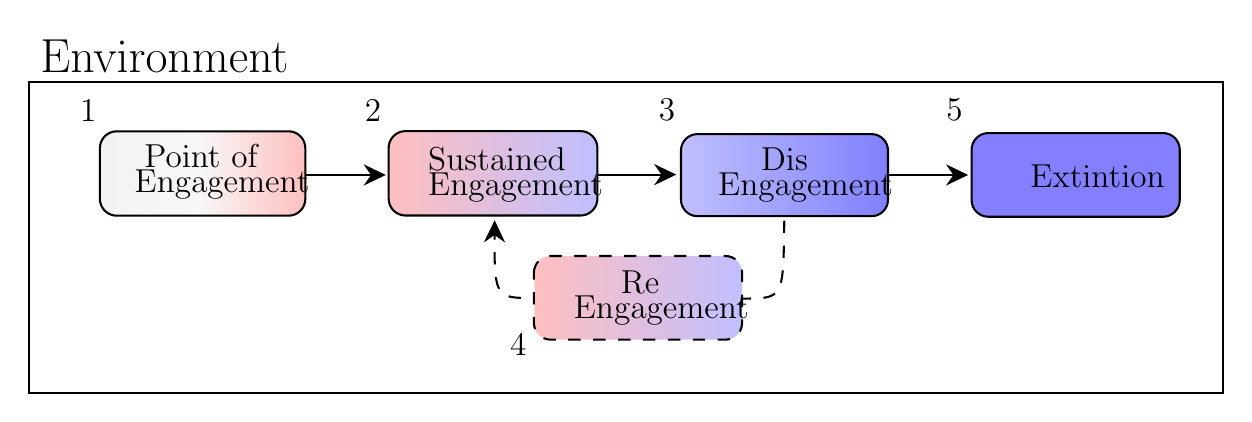
\begin{tikzpicture}[x=0.75pt,y=0.75pt,yscale=-1,xscale=1]
%uncomment if require: \path (0,200); %set diagram left start at 0, and has height of 200

%Shape: Rectangle [id:dp21453085870796063] 
\draw   (14.1,36.6) -- (589.6,36.6) -- (589.6,186.3) -- (14.1,186.3) -- cycle ;
%Rounded Rect [id:dp8669331486657136] 
\path  [shading=_f0h1xn2np,_2yn49zl61,path fading= _gj5ns3oqm ,fading transform={xshift=2}] (48.4,68.36) .. controls (48.4,63.87) and (52.04,60.22) .. (56.53,60.22) -- (139.24,60.22) .. controls (143.73,60.22) and (147.37,63.87) .. (147.37,68.36) -- (147.37,92.76) .. controls (147.37,97.25) and (143.73,100.89) .. (139.24,100.89) -- (56.53,100.89) .. controls (52.04,100.89) and (48.4,97.25) .. (48.4,92.76) -- cycle ; % for fading 
 \draw   (48.4,68.36) .. controls (48.4,63.87) and (52.04,60.22) .. (56.53,60.22) -- (139.24,60.22) .. controls (143.73,60.22) and (147.37,63.87) .. (147.37,68.36) -- (147.37,92.76) .. controls (147.37,97.25) and (143.73,100.89) .. (139.24,100.89) -- (56.53,100.89) .. controls (52.04,100.89) and (48.4,97.25) .. (48.4,92.76) -- cycle ; % for border 

%Straight Lines [id:da4505594811913791] 
\draw    (147.6,81.26) -- (183.16,81.26) ;
\draw [shift={(186.16,81.26)}, rotate = 180] [fill={rgb, 255:red, 0; green, 0; blue, 0 }  ][line width=0.08]  [draw opacity=0] (10.72,-5.15) -- (0,0) -- (10.72,5.15) -- (7.12,0) -- cycle    ;
%Rounded Rect [id:dp29846373438871854] 
\path  [shading=_25n4qjk0b,_5ocf120kv,path fading= _ugfmlo9rg ,fading transform={xshift=2}] (187.51,68.26) .. controls (187.51,63.77) and (191.16,60.13) .. (195.65,60.13) -- (279.95,60.13) .. controls (284.44,60.13) and (288.09,63.77) .. (288.09,68.26) -- (288.09,92.66) .. controls (288.09,97.15) and (284.44,100.8) .. (279.95,100.8) -- (195.65,100.8) .. controls (191.16,100.8) and (187.51,97.15) .. (187.51,92.66) -- cycle ; % for fading 
 \draw   (187.51,68.26) .. controls (187.51,63.77) and (191.16,60.13) .. (195.65,60.13) -- (279.95,60.13) .. controls (284.44,60.13) and (288.09,63.77) .. (288.09,68.26) -- (288.09,92.66) .. controls (288.09,97.15) and (284.44,100.8) .. (279.95,100.8) -- (195.65,100.8) .. controls (191.16,100.8) and (187.51,97.15) .. (187.51,92.66) -- cycle ; % for border 

%Straight Lines [id:da4495263911578298] 
\draw    (288.09,81.1) -- (323.09,81.1) ;
\draw [shift={(326.09,81.1)}, rotate = 180] [fill={rgb, 255:red, 0; green, 0; blue, 0 }  ][line width=0.08]  [draw opacity=0] (10.72,-5.15) -- (0,0) -- (10.72,5.15) -- (7.12,0) -- cycle    ;
%Rounded Rect [id:dp9135925108190124] 
\path  [shading=_03e54ezl1,_daocnbh0q,path fading= _thlshpcj1 ,fading transform={xshift=2}] (328.37,69.49) .. controls (328.37,65.13) and (331.91,61.59) .. (336.28,61.59) -- (420.18,61.59) .. controls (424.55,61.59) and (428.09,65.13) .. (428.09,69.49) -- (428.09,93.21) .. controls (428.09,97.58) and (424.55,101.11) .. (420.18,101.11) -- (336.28,101.11) .. controls (331.91,101.11) and (328.37,97.58) .. (328.37,93.21) -- cycle ; % for fading 
 \draw   (328.37,69.49) .. controls (328.37,65.13) and (331.91,61.59) .. (336.28,61.59) -- (420.18,61.59) .. controls (424.55,61.59) and (428.09,65.13) .. (428.09,69.49) -- (428.09,93.21) .. controls (428.09,97.58) and (424.55,101.11) .. (420.18,101.11) -- (336.28,101.11) .. controls (331.91,101.11) and (328.37,97.58) .. (328.37,93.21) -- cycle ; % for border 

%Rounded Rect [id:dp630049377495355] 
\path  [shading=_qf8n4pbxh,_2e7ef02nx,path fading= _a3543rpu3 ,fading transform={xshift=2}] (257.51,128.36) .. controls (257.51,123.9) and (261.13,120.29) .. (265.58,120.29) -- (349.73,120.29) .. controls (354.19,120.29) and (357.8,123.9) .. (357.8,128.36) -- (357.8,152.55) .. controls (357.8,157.01) and (354.19,160.62) .. (349.73,160.62) -- (265.58,160.62) .. controls (261.13,160.62) and (257.51,157.01) .. (257.51,152.55) -- cycle ; % for fading 
 \draw  [dash pattern={on 4.5pt off 4.5pt}] (257.51,128.36) .. controls (257.51,123.9) and (261.13,120.29) .. (265.58,120.29) -- (349.73,120.29) .. controls (354.19,120.29) and (357.8,123.9) .. (357.8,128.36) -- (357.8,152.55) .. controls (357.8,157.01) and (354.19,160.62) .. (349.73,160.62) -- (265.58,160.62) .. controls (261.13,160.62) and (257.51,157.01) .. (257.51,152.55) -- cycle ; % for border 

%Straight Lines [id:da1505945863891579] 
\draw    (427.92,81.26) -- (463.72,81.26) ;
\draw [shift={(466.72,81.26)}, rotate = 180] [fill={rgb, 255:red, 0; green, 0; blue, 0 }  ][line width=0.08]  [draw opacity=0] (10.72,-5.15) -- (0,0) -- (10.72,5.15) -- (7.12,0) -- cycle    ;
%Rounded Rect [id:dp7652426478992563] 
\draw  [fill={rgb, 255:red, 8; green, 0; blue, 255 }  ,fill opacity=0.5 ] (468.37,69.13) .. controls (468.37,64.68) and (471.98,61.07) .. (476.44,61.07) -- (560.59,61.07) .. controls (565.05,61.07) and (568.66,64.68) .. (568.66,69.13) -- (568.66,93.33) .. controls (568.66,97.79) and (565.05,101.4) .. (560.59,101.4) -- (476.44,101.4) .. controls (471.98,101.4) and (468.37,97.79) .. (468.37,93.33) -- cycle ;
%Curve Lines [id:da6295563644706698] 
\draw  [dash pattern={on 4.5pt off 4.5pt}]  (238.57,106.4) .. controls (238.32,140.92) and (238.67,140.53) .. (257.51,140.53) ;
\draw [shift={(238.6,103.1)}, rotate = 90.44] [fill={rgb, 255:red, 0; green, 0; blue, 0 }  ][line width=0.08]  [draw opacity=0] (10.72,-5.15) -- (0,0) -- (10.72,5.15) -- (7.12,0) -- cycle    ;
%Curve Lines [id:da022545744318036687] 
\draw  [dash pattern={on 4.5pt off 4.5pt}]  (378.14,103.27) .. controls (377.57,140.99) and (378.09,140.81) .. (357.8,140.81) ;

% Text Node
\draw (65.5,23.28) node  [font=\fontsize{0.67em}{0.8em}\selectfont] [align=left] {\begin{minipage}[lt]{68.75pt}\setlength\topsep{0pt}
\begin{center}
{\LARGE Environment}
\end{center}

\end{minipage}};
% Text Node
\draw (97.09,79.56) node  [font=\fontsize{0.67em}{0.8em}\selectfont] [align=left] {\begin{minipage}[lt]{47.87pt}\setlength\topsep{0pt}
\begin{center}
{\large Point of}\\{\large Engagement}
\end{center}

\end{minipage}};
% Text Node
\draw (238.5,80.46) node  [font=\fontsize{0.67em}{0.8em}\selectfont] [align=left] {\begin{minipage}[lt]{47.87pt}\setlength\topsep{0pt}
\begin{center}
{\large Sustained}\\{\large Engagement}
\end{center}

\end{minipage}};
% Text Node
\draw (378.23,81.35) node  [font=\fontsize{0.67em}{0.8em}\selectfont] [align=left] {\begin{minipage}[lt]{47.87pt}\setlength\topsep{0pt}
\begin{center}
{\large Dis}\\{\large Engagement}
\end{center}

\end{minipage}};
% Text Node
\draw (518.51,81.23) node  [font=\fontsize{0.67em}{0.8em}\selectfont] [align=left] {\begin{minipage}[lt]{32.64pt}\setlength\topsep{0pt}
\begin{center}
{\large Extintion}
\end{center}

\end{minipage}};
% Text Node
\draw (308.67,140.46) node  [font=\fontsize{0.67em}{0.8em}\selectfont] [align=left] {\begin{minipage}[lt]{47.87pt}\setlength\topsep{0pt}
\begin{center}
{\large Re}\\{\large Engagement}
\end{center}

\end{minipage}};
% Text Node
\draw (37.33,43.67) node [anchor=north west][inner sep=0.75pt]   [align=left] {{\large 1}};
% Text Node
\draw (174.53,43.67) node [anchor=north west][inner sep=0.75pt]   [align=left] {{\large 2}};
% Text Node
\draw (316.2,43) node [anchor=north west][inner sep=0.75pt]   [align=left] {{\large 3}};
% Text Node
\draw (244.53,156.67) node [anchor=north west][inner sep=0.75pt]   [align=left] {{\large 4}};
% Text Node
\draw (454.73,43) node [anchor=north west][inner sep=0.75pt]   [align=left] {{\large 5}};

\end{tikzpicture}

\end{adjustbox}
\end{center}

\caption[\textbf{Stages of the engagement process mode}]{Solid and dashed lines represent compulsory and  optional paths. Moving from the left to the right we can imagine 1 as being the first interaction that an individual has with an object. This might happen as the result of a prior belief that the object is able to provide a pleasurable experience. The individual will interact with the object for as long as this last one is able to provide a gratifying experience(i.e. stage 2). However, if this is not the case, or constraints from the surrounding environment emerge, the individual will gradually reduce their interaction with the object (i.e. stage 3). At this point we can either observe an alternation between re-engagement and disengagement (i.e. stage 4) or reach an inevitable state of complete withdrawal from the object (i.e. stage 5)}
\label{fig: eng_proc_model_1}
\end{figure}
\paragraph*{Point of engagement} This is the starting point of the engagement process, it is the moment in which the individual’s attention is directed towards a specific object or activity due its properties and capacity to fulfil specific motivational drives.

\paragraph*{Period of engagement} This is the period during which the individual has a sustained interaction with the object of interest. In this case, a situation of sustained and prolonged interaction is conditional on the ability of the object to provide a positive and stimulating experience.

\paragraph*{Disengagement} This stage defines the moment in which the individual reduces the interaction with the object due to internal or external factors. The internal factors are usually connected to loss of interest or pressure derived by the time passing, external factors instead relate more to the inability of the activity to provide a positive experience or to the occurrence of external events in the environment surrounding the individual.

\paragraph*{Re-engagement} It identifies the moment in which the user returns to a sustained level of activity after disengagement occurred. This can happen both in the short and long term and it is the result of positive experiences with the activity, which are usually linked to be exposed to rewarding incentives or novel content within the activity.

\paragraph*{Extinction} In case of prolonged disengagement, marked unsatisfying experiences or impactful external events, the individual might terminate its interactions with the object leaving no further possibility to re-engage with it.

\subsection{From Motivation to Engagement}
\label{eng_reward_motivation}
What emerged from this brief overview of the literature is that engagement seems to be best described as a process controlled by the characteristics of an object, the internal state of the individual interacting with it and eventual environmental factors external to both. In this view engagement appears as a second order factor generated by the internal state of the individual and concerned with the description and quantification  of their interactions with an object  \cite{lucas2004sex,o2008user,jennett2008measuring,boyle2012engagement,connolly2012systematic,csikszentmihalyi2014toward}.The quality and quantity of these interactions seem to be conditional on the ability of the object to provide feelings of enjoyment and pleasure \cite{lucas2004sex,o2008user,jennett2008measuring,boyle2012engagement,connolly2012systematic,csikszentmihalyi2014toward}. We can already see a connection between the construct of engagement and the reward-driven motivational processes presented in section \ref{motivation}, especially if we look at the behavioural level. In the context of videogames, motivational processes seem to pertain the formation and modulation of unobservable (i.e. latent) states characterizing the individual before, during and after the interaction with a videogame. On the other hand, engagement appears to describe the observable aspects of this interaction both at the behavioural and experiential level \cite{lucas2004sex,o2008user,jennett2008measuring,boyle2012engagement,connolly2012systematic,csikszentmihalyi2014toward}. A more clear illustration of this idea is presented in Figure \ref{fig: eng_proc_model_2} 
\begin{figure}[h]
\begin{center}
\begin{adjustbox}{width=\columnwidth}

\tikzset {_tol09vz9c/.code = {\pgfsetadditionalshadetransform{ \pgftransformshift{\pgfpoint{0 bp } { 0 bp }  }  \pgftransformrotate{0 }  \pgftransformscale{2 }  }}}
\pgfdeclarehorizontalshading{_j7rsmr3nr}{150bp}{rgb(0bp)=(0.93,0.93,0.93);
rgb(37.5bp)=(0.93,0.93,0.93);
rgb(62.5bp)=(1,0,0);
rgb(100bp)=(1,0,0)}
\tikzset{_yxq6cdpsj/.code = {\pgfsetadditionalshadetransform{\pgftransformshift{\pgfpoint{0 bp } { 0 bp }  }  \pgftransformrotate{0 }  \pgftransformscale{2 } }}}
\pgfdeclarehorizontalshading{_7yg524gtp} {150bp} {color(0bp)=(transparent!75);
color(37.5bp)=(transparent!75);
color(62.5bp)=(transparent!75);
color(100bp)=(transparent!75) } 
\pgfdeclarefading{_y4z1b8bbb}{\tikz \fill[shading=_7yg524gtp,_yxq6cdpsj] (0,0) rectangle (50bp,50bp); } 

% Gradient Info
  
\tikzset {_3ywdqyfah/.code = {\pgfsetadditionalshadetransform{ \pgftransformshift{\pgfpoint{0 bp } { 0 bp }  }  \pgftransformrotate{0 }  \pgftransformscale{2 }  }}}
\pgfdeclarehorizontalshading{_2t0kw1fpw}{150bp}{rgb(0bp)=(1,0,0);
rgb(37.5bp)=(1,0,0);
rgb(62.5bp)=(0,0,1);
rgb(100bp)=(0,0,1)}
\tikzset{_yvsljnreh/.code = {\pgfsetadditionalshadetransform{\pgftransformshift{\pgfpoint{0 bp } { 0 bp }  }  \pgftransformrotate{0 }  \pgftransformscale{2 } }}}
\pgfdeclarehorizontalshading{_fpvhgjdei} {150bp} {color(0bp)=(transparent!75);
color(37.5bp)=(transparent!75);
color(62.5bp)=(transparent!75);
color(100bp)=(transparent!75) } 
\pgfdeclarefading{_y32y00acn}{\tikz \fill[shading=_fpvhgjdei,_yvsljnreh] (0,0) rectangle (50bp,50bp); } 

% Gradient Info
  
\tikzset {_k82gbaai2/.code = {\pgfsetadditionalshadetransform{ \pgftransformshift{\pgfpoint{0 bp } { 0 bp }  }  \pgftransformrotate{0 }  \pgftransformscale{2 }  }}}
\pgfdeclarehorizontalshading{_mzd6axxaa}{150bp}{rgb(0bp)=(0,0,1);
rgb(37.5bp)=(0,0,1);
rgb(62.5bp)=(0,0,1);
rgb(100bp)=(0,0,1)}
\tikzset{_1ih9fwhej/.code = {\pgfsetadditionalshadetransform{\pgftransformshift{\pgfpoint{0 bp } { 0 bp }  }  \pgftransformrotate{0 }  \pgftransformscale{2 } }}}
\pgfdeclarehorizontalshading{_py52u7ab2} {150bp} {color(0bp)=(transparent!75);
color(37.5bp)=(transparent!75);
color(62.5bp)=(transparent!50);
color(100bp)=(transparent!50) } 
\pgfdeclarefading{_wr0vkxl3y}{\tikz \fill[shading=_py52u7ab2,_1ih9fwhej] (0,0) rectangle (50bp,50bp); } 

% Gradient Info
  
\tikzset {_3kvg59946/.code = {\pgfsetadditionalshadetransform{ \pgftransformshift{\pgfpoint{0 bp } { 0 bp }  }  \pgftransformrotate{-90 }  \pgftransformscale{2 }  }}}
\pgfdeclarehorizontalshading{_wvh4fdo7p}{150bp}{rgb(0bp)=(1,0,0);
rgb(37.5bp)=(1,0,0);
rgb(62.5bp)=(0,0,1);
rgb(100bp)=(0,0,1)}
\tikzset{_dv8t3n3dv/.code = {\pgfsetadditionalshadetransform{\pgftransformshift{\pgfpoint{0 bp } { 0 bp }  }  \pgftransformrotate{-90 }  \pgftransformscale{2 } }}}
\pgfdeclarehorizontalshading{_abfcxja44} {150bp} {color(0bp)=(transparent!75);
color(37.5bp)=(transparent!75);
color(62.5bp)=(transparent!75);
color(100bp)=(transparent!75) } 
\pgfdeclarefading{_tndnn1d2b}{\tikz \fill[shading=_abfcxja44,_dv8t3n3dv] (0,0) rectangle (50bp,50bp); } 

% Gradient Info
  
\tikzset {_475pso13i/.code = {\pgfsetadditionalshadetransform{ \pgftransformshift{\pgfpoint{0 bp } { 0 bp }  }  \pgftransformrotate{-90 }  \pgftransformscale{2 }  }}}
\pgfdeclarehorizontalshading{_f5gjc5tzr}{150bp}{rgb(0bp)=(0,0,1);
rgb(37.5bp)=(0,0,1);
rgb(62.5bp)=(1,0,0);
rgb(100bp)=(1,0,0)}
\tikzset{_fwuteqqte/.code = {\pgfsetadditionalshadetransform{\pgftransformshift{\pgfpoint{0 bp } { 0 bp }  }  \pgftransformrotate{-90 }  \pgftransformscale{2 } }}}
\pgfdeclarehorizontalshading{_gbjam9yyh} {150bp} {color(0bp)=(transparent!75);
color(37.5bp)=(transparent!75);
color(62.5bp)=(transparent!75);
color(100bp)=(transparent!75) } 
\pgfdeclarefading{_wo5obn5gu}{\tikz \fill[shading=_gbjam9yyh,_fwuteqqte] (0,0) rectangle (50bp,50bp); } 
\tikzset{every picture/.style={line width=0.75pt}} %set default line width to 0.75pt        

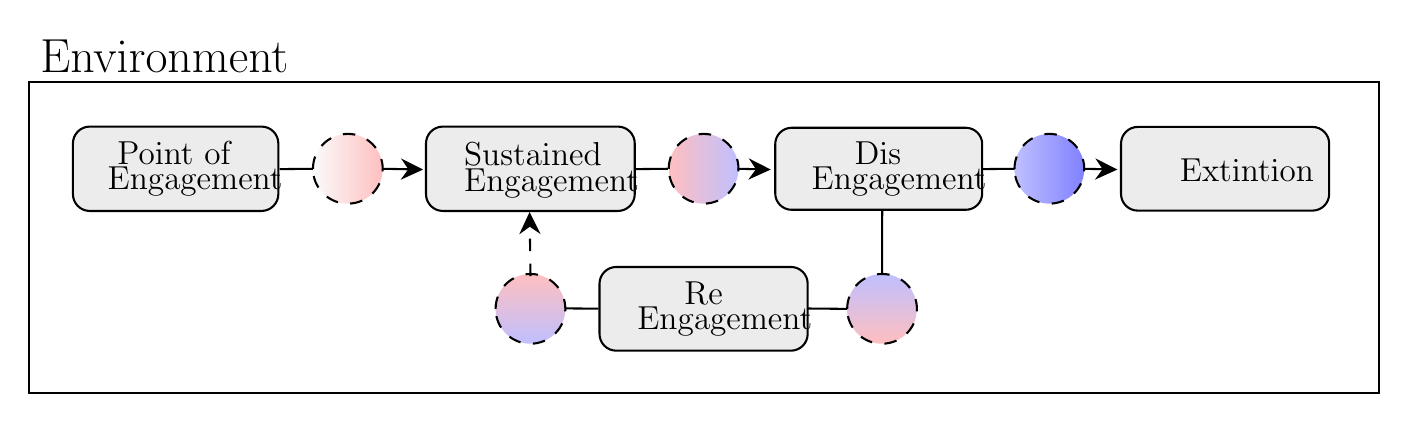
\begin{tikzpicture}[x=0.75pt,y=0.75pt,yscale=-1,xscale=1]
%uncomment if require: \path (0,357); %set diagram left start at 0, and has height of 357

%Rounded Rect [id:dp08887598870261693] 
\draw  [fill={rgb, 255:red, 236; green, 236; blue, 236 }  ,fill opacity=1 ] (30.4,81.08) .. controls (30.4,76.59) and (34.04,72.95) .. (38.53,72.95) -- (121.24,72.95) .. controls (125.73,72.95) and (129.37,76.59) .. (129.37,81.08) -- (129.37,105.48) .. controls (129.37,109.97) and (125.73,113.61) .. (121.24,113.61) -- (38.53,113.61) .. controls (34.04,113.61) and (30.4,109.97) .. (30.4,105.48) -- cycle ;
%Rounded Rect [id:dp06222122397376195] 
\draw  [fill={rgb, 255:red, 236; green, 236; blue, 236 }  ,fill opacity=1 ] (200.51,81.08) .. controls (200.51,76.59) and (204.16,72.95) .. (208.65,72.95) -- (292.95,72.95) .. controls (297.44,72.95) and (301.09,76.59) .. (301.09,81.08) -- (301.09,105.48) .. controls (301.09,109.97) and (297.44,113.61) .. (292.95,113.61) -- (208.65,113.61) .. controls (204.16,113.61) and (200.51,109.97) .. (200.51,105.48) -- cycle ;
%Rounded Rect [id:dp7821816318063516] 
\draw  [fill={rgb, 255:red, 236; green, 236; blue, 236 }  ,fill opacity=1 ] (368.77,81.42) .. controls (368.77,77.06) and (372.31,73.52) .. (376.68,73.52) -- (460.58,73.52) .. controls (464.95,73.52) and (468.49,77.06) .. (468.49,81.42) -- (468.49,105.14) .. controls (468.49,109.5) and (464.95,113.04) .. (460.58,113.04) -- (376.68,113.04) .. controls (372.31,113.04) and (368.77,109.5) .. (368.77,105.14) -- cycle ;
%Rounded Rect [id:dp20372970008362923] 
\draw  [fill={rgb, 255:red, 236; green, 236; blue, 236 }  ,fill opacity=1 ] (535.37,81.18) .. controls (535.37,76.73) and (538.98,73.12) .. (543.44,73.12) -- (627.59,73.12) .. controls (632.05,73.12) and (635.66,76.73) .. (635.66,81.18) -- (635.66,105.38) .. controls (635.66,109.83) and (632.05,113.44) .. (627.59,113.44) -- (543.44,113.44) .. controls (538.98,113.44) and (535.37,109.83) .. (535.37,105.38) -- cycle ;
%Shape: Circle [id:dp19552380180112794] 
\path  [shading=_j7rsmr3nr,_tol09vz9c,path fading= _y4z1b8bbb ,fading transform={xshift=2}] (146.05,93.28) .. controls (146.05,84) and (153.57,76.48) .. (162.85,76.48) .. controls (172.13,76.48) and (179.65,84) .. (179.65,93.28) .. controls (179.65,102.56) and (172.13,110.08) .. (162.85,110.08) .. controls (153.57,110.08) and (146.05,102.56) .. (146.05,93.28) -- cycle ; % for fading 
 \draw  [dash pattern={on 4.5pt off 4.5pt}] (146.05,93.28) .. controls (146.05,84) and (153.57,76.48) .. (162.85,76.48) .. controls (172.13,76.48) and (179.65,84) .. (179.65,93.28) .. controls (179.65,102.56) and (172.13,110.08) .. (162.85,110.08) .. controls (153.57,110.08) and (146.05,102.56) .. (146.05,93.28) -- cycle ; % for border 

%Shape: Circle [id:dp27430889542654724] 
\path  [shading=_2t0kw1fpw,_3ywdqyfah,path fading= _y32y00acn ,fading transform={xshift=2}] (317.46,93.28) .. controls (317.46,84) and (324.98,76.48) .. (334.26,76.48) .. controls (343.54,76.48) and (351.06,84) .. (351.06,93.28) .. controls (351.06,102.56) and (343.54,110.08) .. (334.26,110.08) .. controls (324.98,110.08) and (317.46,102.56) .. (317.46,93.28) -- cycle ; % for fading 
 \draw  [dash pattern={on 4.5pt off 4.5pt}] (317.46,93.28) .. controls (317.46,84) and (324.98,76.48) .. (334.26,76.48) .. controls (343.54,76.48) and (351.06,84) .. (351.06,93.28) .. controls (351.06,102.56) and (343.54,110.08) .. (334.26,110.08) .. controls (324.98,110.08) and (317.46,102.56) .. (317.46,93.28) -- cycle ; % for border 

%Rounded Rect [id:dp4578454458037269] 
\draw  [fill={rgb, 255:red, 236; green, 236; blue, 236 }  ,fill opacity=1 ] (284.11,148.66) .. controls (284.11,144.2) and (287.73,140.59) .. (292.18,140.59) -- (376.33,140.59) .. controls (380.79,140.59) and (384.4,144.2) .. (384.4,148.66) -- (384.4,172.85) .. controls (384.4,177.31) and (380.79,180.92) .. (376.33,180.92) -- (292.18,180.92) .. controls (287.73,180.92) and (284.11,177.31) .. (284.11,172.85) -- cycle ;
%Shape: Circle [id:dp8141702965644008] 
\path  [shading=_mzd6axxaa,_k82gbaai2,path fading= _wr0vkxl3y ,fading transform={xshift=2}] (484.05,93.28) .. controls (484.05,84) and (491.57,76.48) .. (500.85,76.48) .. controls (510.13,76.48) and (517.65,84) .. (517.65,93.28) .. controls (517.65,102.56) and (510.13,110.08) .. (500.85,110.08) .. controls (491.57,110.08) and (484.05,102.56) .. (484.05,93.28) -- cycle ; % for fading 
 \draw  [dash pattern={on 4.5pt off 4.5pt}] (484.05,93.28) .. controls (484.05,84) and (491.57,76.48) .. (500.85,76.48) .. controls (510.13,76.48) and (517.65,84) .. (517.65,93.28) .. controls (517.65,102.56) and (510.13,110.08) .. (500.85,110.08) .. controls (491.57,110.08) and (484.05,102.56) .. (484.05,93.28) -- cycle ; % for border 

%Shape: Circle [id:dp5389996328417695] 
\path  [shading=_wvh4fdo7p,_3kvg59946,path fading= _tndnn1d2b ,fading transform={xshift=2}] (234.05,160.76) .. controls (234.05,151.48) and (241.57,143.96) .. (250.85,143.96) .. controls (260.13,143.96) and (267.65,151.48) .. (267.65,160.76) .. controls (267.65,170.03) and (260.13,177.56) .. (250.85,177.56) .. controls (241.57,177.56) and (234.05,170.03) .. (234.05,160.76) -- cycle ; % for fading 
 \draw  [dash pattern={on 4.5pt off 4.5pt}] (234.05,160.76) .. controls (234.05,151.48) and (241.57,143.96) .. (250.85,143.96) .. controls (260.13,143.96) and (267.65,151.48) .. (267.65,160.76) .. controls (267.65,170.03) and (260.13,177.56) .. (250.85,177.56) .. controls (241.57,177.56) and (234.05,170.03) .. (234.05,160.76) -- cycle ; % for border 

%Shape: Circle [id:dp655926787503073] 
\path  [shading=_f5gjc5tzr,_475pso13i,path fading= _wo5obn5gu ,fading transform={xshift=2}] (403.43,160.76) .. controls (403.43,151.48) and (410.95,143.96) .. (420.23,143.96) .. controls (429.51,143.96) and (437.03,151.48) .. (437.03,160.76) .. controls (437.03,170.03) and (429.51,177.56) .. (420.23,177.56) .. controls (410.95,177.56) and (403.43,170.03) .. (403.43,160.76) -- cycle ; % for fading 
 \draw  [dash pattern={on 4.5pt off 4.5pt}] (403.43,160.76) .. controls (403.43,151.48) and (410.95,143.96) .. (420.23,143.96) .. controls (429.51,143.96) and (437.03,151.48) .. (437.03,160.76) .. controls (437.03,170.03) and (429.51,177.56) .. (420.23,177.56) .. controls (410.95,177.56) and (403.43,170.03) .. (403.43,160.76) -- cycle ; % for border 

%Shape: Rectangle [id:dp8053989914309859] 
\draw   (9.1,51.6) -- (659.6,51.6) -- (659.6,201.3) -- (9.1,201.3) -- cycle ;
%Straight Lines [id:da46348057228029615] 
\draw    (130,93.45) -- (146.05,93.28) ;
%Straight Lines [id:da06616438858203633] 
\draw    (179.65,93.28) -- (196.1,93.59) ;
\draw [shift={(199.1,93.65)}, rotate = 181.09] [fill={rgb, 255:red, 0; green, 0; blue, 0 }  ][line width=0.08]  [draw opacity=0] (10.72,-5.15) -- (0,0) -- (10.72,5.15) -- (7.12,0) -- cycle    ;
%Straight Lines [id:da6977755883492565] 
\draw    (350.65,93.28) -- (363.6,93.58) ;
\draw [shift={(366.6,93.65)}, rotate = 181.33] [fill={rgb, 255:red, 0; green, 0; blue, 0 }  ][line width=0.08]  [draw opacity=0] (10.72,-5.15) -- (0,0) -- (10.72,5.15) -- (7.12,0) -- cycle    ;
%Straight Lines [id:da47311877150256343] 
\draw    (301,93.45) -- (317.05,93.28) ;
%Straight Lines [id:da21451072469562127] 
\draw    (468,93.45) -- (484.05,93.28) ;
%Straight Lines [id:da7997515132020875] 
\draw    (517.65,93.28) -- (530.6,93.58) ;
\draw [shift={(533.6,93.65)}, rotate = 181.33] [fill={rgb, 255:red, 0; green, 0; blue, 0 }  ][line width=0.08]  [draw opacity=0] (10.72,-5.15) -- (0,0) -- (10.72,5.15) -- (7.12,0) -- cycle    ;
%Straight Lines [id:da5942266070774226] 
\draw    (420.23,143.98) -- (420.32,112.84) ;
%Straight Lines [id:da1853788628800106] 
\draw  [dash pattern={on 4.5pt off 4.5pt}]  (250.85,144.98) -- (250.47,117.1) ;
\draw [shift={(250.42,114.1)}, rotate = 89.2] [fill={rgb, 255:red, 0; green, 0; blue, 0 }  ][line width=0.08]  [draw opacity=0] (10.72,-5.15) -- (0,0) -- (10.72,5.15) -- (7.12,0) -- cycle    ;
%Straight Lines [id:da47123825108915496] 
\draw    (403.43,160.78) -- (384.32,160.6) ;
%Straight Lines [id:da3253725947262416] 
\draw    (283.52,160.68) -- (267.65,160.55) ;

% Text Node
\draw (334.26,160.76) node  [font=\fontsize{0.67em}{0.8em}\selectfont] [align=left] {\begin{minipage}[lt]{47.87pt}\setlength\topsep{0pt}
\begin{center}
{\large Re}\\{\large Engagement}
\end{center}

\end{minipage}};
% Text Node
\draw (79.09,93.28) node  [font=\fontsize{0.67em}{0.8em}\selectfont] [align=left] {\begin{minipage}[lt]{47.87pt}\setlength\topsep{0pt}
\begin{center}
{\large Point of}\\{\large Engagement}
\end{center}

\end{minipage}};
% Text Node
\draw (60.5,38.28) node  [font=\fontsize{0.67em}{0.8em}\selectfont] [align=left] {\begin{minipage}[lt]{68.75pt}\setlength\topsep{0pt}
\begin{center}
{\LARGE Environment}
\end{center}

\end{minipage}};
% Text Node
\draw (418.23,93.28) node  [font=\fontsize{0.67em}{0.8em}\selectfont] [align=left] {\begin{minipage}[lt]{47.87pt}\setlength\topsep{0pt}
\begin{center}
{\large Dis}\\{\large Engagement}
\end{center}

\end{minipage}};
% Text Node
\draw (585.51,93.28) node  [font=\fontsize{0.67em}{0.8em}\selectfont] [align=left] {\begin{minipage}[lt]{32.64pt}\setlength\topsep{0pt}
\begin{center}
{\large Extintion}
\end{center}

\end{minipage}};
% Text Node
\draw (250.8,93.28) node  [font=\fontsize{0.67em}{0.8em}\selectfont] [align=left] {\begin{minipage}[lt]{47.87pt}\setlength\topsep{0pt}
\begin{center}
{\large Sustained}\\{\large Engagement}
\end{center}

\end{minipage}};
\end{tikzpicture}

\end{adjustbox}
\end{center}
\caption{\textbf{Diagram summarizing the different stages of the engagement process mode introducing the contribution of environment and latent states}.}
\label{fig: eng_proc_model_2}
\end{figure}
Here we adapted the engagement process model of O'Brien and colleagues \cite{o2008user} presented in Figure \ref{fig: eng_proc_model_1} incorporating the state of the individual. In this view, the motivational state of an individual precede (on an arbitrary temporal scale) and contribute at determining in which phase of the engagement process an individual will be located when interacting with as specific object (i.e. a videogame) again in the future. This implies that, at any point in time, the history of observed engagement indicators (e.g. frequency and amount of interactions) can provide information on the current unobservable motivational state of the individual. In section \ref{motivation_hist} we specified that the motivational propensity that an individual might have towards a certain object is in part determined by the rewarding properties of the object itself \cite{berridge2004motivation}. But how would these properties look in the context of a videogame? Surely playing videogames is not relevant for satisfying fundamental physiological needs nor it is directly linked to other type of powerful reinforcers (e.g. money). In this case, the distinction between primary and secondary rewards made in section \ref{motivation_hist} becomes particularly useful for understating the framework in which videogames lies: what acts as a reinforcer during the playing behaviour are the structural characteristics defining the videogame itself \cite{king2010role, king2010video, yannakakis2013player}. We will better define the concept of videogame structural characteristics later on but for now we can think of them as any type of in-game element that an individual might interact with during the playing behaviour \cite{king2010role,king2010video}. None of these structural characteristics are intrinsically rewarding, but they can become so over time, through conventional learning processes, if they are able to provide pleasurable experiences to the individual \cite{skinner1953science, berridge2004motivation, przybylski2010motivational}. In a dynamic fashion, interacting with specific features in the videogame might produce positive reactions in the individual and make new interactions more probable. In this view engagement can be seen as the observable manifestation of the unobservable motivational propensity that an individual has towards a specific videogame. In other words, we can think of engagement as the behavioural realisation of a motivational process aimed at maximizing the positive experiences provided by the in-game elements. 

\subsection{Videogames Structural Characteristics}
\label{factors_engagement}
It should be evident by now that the ability to construct videogames with effective rewarding characteristics is of pivotal importance for generating and sustaining engagement \cite{king2010role, king2010video, yannakakis2013player}. Various attempt has been made to build a taxonomy of these characteristics, King et al. \cite{king2010video} for instance outlined a series of features that effective videogames structural characteristics should have. These are: social features, manipulation (e.g. crafting) feature, narrative features, achievement and punishing features and aesthetic features. Westwood et al. \cite{westwood2010role} were able to use this taxonomy for effectively individuating which specific structural characteristic were driving playing behaviour in a group of videogame players. The taxonomy provided by King et al., although exhaustive, provides a descriptive rather than mechanistic account of the structural characteristic driving playing behaviour \cite{king2010role}. Adopting a different approach, Wang and Sun proposed to frame the work of King et al. in terms of reinforcers \cite{king2010video, wang2011game}. In this view, playing behaviour in different games is sustained by different reinforcing mechanics covering the areas described by King et al. \cite{king2010video, wang2011game}. Among these mechanics there are: scoring systems, in-game items and resources, achievements systems, feedback messages, animation events and the unlocking of new game contents \cite{wang2011game}. The authors also described a series of attributed that the in-game rewards should have for being effective: they need to possess social value within a shared environment, they need to have visible effects within the game world and they need time and effort for being obtained \cite{wang2011game}. Extending the work of Wang and Sun, Philips and colleagues focused on a description of the temporal characteristics that in-game reinforcers may possess, namely being limited in duration, transient and context dependent, permanent or consumable \cite{phillips2013videogame}. A connected although separate stream of research tried to categorize which elements inside a videogame might produce pleasurable experiences for the players however focusing more on the characteristics of the individuals rather than those of the game itself. Similarly to trait theories in psychology, this approach assume that different individual have static, consistent and well defined preferences for some aspects (i.e. structural characteristics). of the playing experience. In his seminal work Bartle tried to identify different approaches that players might have had in playing Multi User Dungeons (MUDs), an early version of the modern Massively Multiplayer Online Role Playing Games (MMORPGs) \cite{bartle1996hearts}. Projecting the players’ attitudes towards the game on two axis: oriented towards action or interaction and oriented towards the game world or the players, Bartle proposed four mutually exclusive categories \cite{bartle1996hearts}. 
\begin{table}[h]
\caption{\textbf{Bartle Taxonomy}}
\label{bartle}
\begin{tabularx}{\textwidth}{|l|X|}
\hline
Achievers   & Action oriented towards the game world. Players interested in mastering the game, aiming to build a status within the game towards their interaction with the environment.                      \\ \hline
Socializers & Interaction with other players. Players driven by the perspective of interacting with other players, deriving satisfaction from their friendship, contacts and social influence within the game \\ \hline
Explorers   & Interaction with the game world. Players aiming to be surprised by the game world, seeking the stimulation derived by the discovery of new areas and the acquisition of knowledge.              \\ \hline
Killers     & Action oriented towards other players. Players interested in demonstrating their superiority over other players posing great value on the reputation obtained through in-game fighting skills.  \\ \hline
\end{tabularx}
\end{table}
Despite this early formulation only considers a specific subset of games and lacks any kind of empirical validation, Bartle's work was the starting point for most of the later efforts on the subject \cite{bartle1996hearts}. Brtle's taxonomy was built on assumptions that were never tested and the proposed categories showed a certain degree of inter-correlation. For this reason Yee tried to develop a methodology for assessing the players’ tendencies towards specific game characteristics \cite{yee2006motivations}. After gathering information from a large sample of players and performing a first round of dimensionality reduction, 10 major factors emerged, these were then condensed in 3 additional facets performing an ulterior round of dimensionality reduction over the previously obtained components \cite{yee2006motivations}. The three main factors that emerged were: 
\begin{table}[h]
\caption{\textbf{Yee Taxonomy}}
\label{yee}
\begin{tabularx}{\textwidth}{|l|X|}
\hline
Achievement & Factor indicating a tendency towards advancing in the game, exploiting its mechanics or competing with it.                           \\ \hline
Social      & Factor indicating a preference for those game characteristics centred on socializing, creating relationship and developing teamwork. \\ \hline
Immersion   & Factor  represents the drive towards the discovery, role-playing and customization mechanics of the game.                            \\ \hline
\end{tabularx}
\end{table}
The model proposed by Yee introduced two interesting variations on what has been done by Bartle: the components are not necessarily mutually exclusive and the focus is shifted from a characterization of the players to a characterization of the in-game elements with which the individuals interact \cite{bartle1996hearts,yee2006motivations}. Despite these improvements, the focus was still on a specific game genre and heavily relied on static and potentially biased measures (i.e. self-report). In order to overcome the limitations of a taxonomy heavily influenced by a specific game genre, Nacke et al. developed a more comprehensive system with the intent to capture the players’ preferences for particular game mechanics regardless of the genre \cite{nacke2011brainhex}. The categories proposed by this model were: 
\begin{table}[h]
\caption{\textbf{BrainHex Taxonomy}}
\label{nacke}
\begin{tabularx}{\textwidth}{|l|X|}
\hline
Seekers     & Players driven by in game mechanics which produces interest and satisfy curiosity..                                                    \\ \hline
Daredevils  & Players motivated by the thrill derived from taking risks in the game.                                                                 \\ \hline
Masterminds & Players who enjoys solving puzzles and finding the best strategies to adopt within the game.                                           \\ \hline
Conquerors  & Players who derive satisfaction from overcoming the challenges provided by the game and from the struggles characterizing the process. \\ \hline
Socializers & Players driven by the interaction with other players.                                                                                  \\ \hline
Achievers   & Players driven by reaching long term goals, often aiming to fully complete the game.                                                   \\ \hline
Survivors   & Players driven by thrilling experiences provided by the game and by the ability of the game environment to generate arousal.           \\ \hline
\end{tabularx}
\end{table}
This formulation appear to have a higher level of details than the approaches of Yee and Bartle, however the number of considered factors grows proportional with the number of game characteristics taken into consideration \cite{nacke2011brainhex}. We won't expand on the supposed link between facets, "neurobiology" and personality components proposed by the authors. The first is purely anecdotal, not supported by any evidence and adopt a conceptualization of the human brain that is, at the very least, primitive \cite{nacke2011brainhex}. Evaluating the relationship between the facets and personality traits could have been an interesting angle to explore, but the use of the infamous Mayers-Briggs model of personality \cite{boyle1995myers} makes the results hard to interpret.


A MODEL INFORMED BY PSYCHOLOGY
What has been illustrated so far show how most the model aiming to address motivational factors in videogames arises directly for the videogame field itself. Using a different approach [4] employed a psychological model for explaining in an empirical way the process through which videogames drive sustained engagement. The underlying idea was that videogames, lacking in the presence of external incentives, provide appeal via the inherent properties of the playing experience. In the original formulation by [3] humans are driven in their every-day life by the satisfaction of basic needs, these results as more effective motivational factors than any kind of  external incentives. We will now present how the formulation by [3] has been employed by [4] for describing gaming mechanics able to promote engagement through the satisfaction of the aforementioned basic needs.
Competence need 
The satisfaction of this need can be provided balancing the ratio between game difficulty and player skill in such a way that the player is placed half way between being bored and overwhelmed by the game, in other words the player needs to feel competent while they play [4]. Despite being a rightful point, the aforementioned process does not describe a motivational factor, but rather the best way through which a player can be introduced to the in-game elements that might act as motivational factors. If a game is too difficult it constitutes an entry barrier while if it’s too easy it might fail to sufficiently engage the user. Moreover, this consideration doesn’t take into account games that, by design, aims to be very difficult (e.g. triggering the need for a challenge) or very easy (e.g. heavily story driven games).
Autonomy need 	
The satisfaction of this need can be provided allowing the players to advance through different challenges and shape the game world in accordance to their will, in this way the players are allowed to act with freedom within the game.
Relatedness need 
The satisfaction of this need can be achieved though the social interactions within the game. A good example of how satisfying this need can increase the motivation to play are games having multiplayer mechanics as core features which are notoriously able to successfully engage large audiences. 
Mastery of controls
The satisfaction of this need can be provided allowing the player to master the controls of the game, this put the players in the position to experience a sense of control and receive appropriated feedbacks from the game, indeed complex mechanics are usually not enjoyed by players as they are seen as a price of admission. Again here the focus seems to be on usability rather than on defining motivational factors. Complicated controls may constitute a barrier preventing some players to experience the game while simple controls allows a larger pool of people to . If we look at some of the most engaging games available, the complexity of the controls range from very simple (e.g. swiping a finger on a screen) to extremely complex (e.g. managing combinations of multiple keys with high temporal constrains).
One of the core point in [4] is that when an activity puts pressure on achieving rewards and avoiding punishments it fosters extrinsic motivation, with potential negative effect on engagement. However, the aforementioned statement seems to be contradicted by the characteristics of some of the most captivating videogames titles, which poses a strong accent on both rewards (i.e. mobile puzzle games) and punishments (e.g. souls-like games or Multiplayer Online Battle Arenas). We won’t go into the merit if the chosen model is a good approximation for the motivational process in humans, but what we can highlight is how its application to the videogame context seems to address more usability issues rather than identifying the presence of motivational factors in games. Despite [4] made an effort for creating a bridge between psychology and the game studies, the result differently from the aforementioned models seems to ‘force’ the theoretical point of view found in [3] to a system (i.e. videogames) without knowing or taking in consideration the characteristics of this last one.
What the works presented so far show is that each different videogame could be considered as an instantiation of a particular virtual environment with proper structural characteristics (i.e. in-game features) and rules (i.e. games mechanics). The player voluntary chose to be an individual in this ‘simulated’ environment, with supposedly no external factors forcing him to stay and behave inside it. Therefore, the question is, what drives their propensity to engage in activities inside the game world? From the work of [19, 38, 39] we saw that there are a series of motivational factors able to account for that and that this factors might be well reflected in the the structural characteristics individuated by [9, 10, 11]. At this point, we might use the theoretical framework provided early on and speculating that an individual, after voluntarily entering the game world, will interact qualitatively and quantitatively with those game features able to act as motivational factors, or in other words, with those features able to provide a pleasurable experience in that particular point in time.


SUMMARY, PROS AND CONS
From this brief overview of some of the works trying to describe the motivational pulls of videogames, we can observe that there is no consensus over a specific taxonomy or theoretical approach. However, some common features among the various models can be observed:
1.	A motivational factor usually has the capacity to generate positive reactions in the player
2.	A motivational factor usually can be individuated in the in game activity in which a player engage the most
3.	There seems to be some common factors across various models: achievement, socialization, exploration and fighting. However this might well be an artefact derived by most of the models having a common ancestor (i.e. [38]) and being influenced by each other.
The relative incongruence among the theoretical approaches present in the literature is that each one tries to find an unified theory for describing a phenomena which is extremely prone to variability: models developed between different game genres (and even within the same genre) my result highly inconsistent due to the different characteristics of each game. Moreover, another critical point is the absence of a solid ‘anchor point’ from which the model can be developed (e.g. how in psychology there is a relatively accepted definition of the personality construct).
These theoretical approaches has a series of advantages:   
1.	They focus on videogames taking in consideration their peculiar characteristics
2.	They have been developed within the area of videogame studies, serving the purpose of providing explanatory models to researchers and professionals who works in the field.
As well as disadvantages:
1.	They are often heavily dependent on specific videogames genres
2.	They seem difficult to generalize across different games
3.	They assume a static conceptualization of motivation than differently from other psychological constructs (i.e. personality) is inherently dynamic
4.	There is very little empirical work done for validating each model

\section{Measuring Motivation and Engagement}
\label{measuring_motivation_engagement}
Now we will illustrate some of the measures that can be employed for evaluating and characterizing the engagement process in videogame players. An in-depth description of this methods would be out of scope for this review so we will limit to a general description outlining advantages and disadvantages for each measuring technique.
    \subsection{Self-report Measures}
    \label{self_report}
    These measures include all those techniques requiring individuals to report their experiences and personal, psychological or demographical characteristics, they require a voluntary and cognitively elaborated answer from the individual and usually aim to measure static/stable attributes. Questionnaires require people to answer a set of questions supposedly indicative of a latent construct that an experimenter wants to measure. They are often employed because supposedly simple, easy to administer and highly scalable, moreover when compared to other kind of measures they offer the possibility to investigate a large set of constructs; that said, some important and major limitations need to be pointed out. Questionnaires often require a cognitive appraisal of actions, emotions or attitudes that despite being essential is not always accessible or able to precisely describe situations in which there is no complete awareness of the motives behind a set of actions [18]. In this view is important to say that conscious appraisal and actual experience may interact or overlap but often don’t coincide [12]. In this view it has to be reported that many attempts in correlating game behaviour and the result to psychometrics tests often produced fragmented and inconclusive findings [29]. A possible reason for this may be the nature of the employed questionnaire, not developed for assessing the characteristics of an individual within a ‘simulation’ of the real world and therefore not being able to describe the in-game behaviour [5]. Some questionnaire for addressing game specific constructs are present in the literature [19, 20] but other than carrying similar problem in explaining the player behaviour they don’t report extensive validation procedures as it is often required for the creation of psychological questionnaires. A series of other limitations affect the employment of questionnaires [21], the adherence of the respondents to social desirability norms, erroneous interpretation of the questions, untruthful answers, constrains in the possible answers, random or systematic measurement errors and in case of mass administrations (i.e. mailing or online recruiting) poor sampling control.
    \subsection{Psychophisiological Measures}
    \label{psychophisio}
    Questionnaires should be able to describe the psychological aspects of the player but are static indices prone to bias or systematic measurement error. On the other hand behavioural measures can account for external manifestations of the player experience in a more objective and naturalistic way but lack in the ability to represent the internal state of the player. As a mediation between this two poles we can pose the measurement of the physiological activity as a proxy for psychological processes (i.e. psychophysiological measures), the core assumption here is that particular physiological responses from the body are linked to basic emotions and cognitive processes [5, 23]. This kind of measures can be derived from a set of techniques ranging from more basic and general (e.g. skin conductance, Electrocardiogram) to more sophisticated and specific ones (e.g. Electroencephalogram, Functional Magnetic Resonance Imaging). The application of psychophysiological measures in a videogame context arises from the assumption that what happens in the game alters the players’ psychological state which in response may affect the body’s physiological response.  Monitoring such body alterations during a game session can assist in reconstructing the player experience [24] as well as in producing more rich players’ profiles and models [5]. Despite being powerful and precise indices for physiological manifestations, their applicability is damped by a series of limitations: they are often perceived as invasive by the individuals [5], depending on the employed hardware they might be expensive, they require particular care in the recording phase, they are extremely prone to artefacts, the signal pre-processing is often a long and laborious activity, their interpretability may be difficult if not a priori hypothesis are formulated, they often require appropriated and minimalistic experimental designs for controlling confounds and investigating only variables of interest [25].
    \subsection{Behavioural Measures}
    \label{behavioural_indices}
    
    
    The works presented so far were concerned mostly with providing a taxonomy for describing different types of videogames structural characteristics. Cowley and colleagues took this a step further proposing a methodology based on in-game behaviour for evaluating which specific in-game elements were driving engagement \cite{cowley2016behavlets}. The underlying idea was that the actions performed by a player within a videogame could be grouped in three different categories depending on their goal (a similar approach can be found in \cite{bartle1996hearts}): social (directed towards other players), achievement (directed towards in-game goals) and fantasy (directed towards escapism). In this view, analyzing the type of actions taken by the player could provide an indication of the underlying factors driving the engagement \cite{cowley2016behavlets}. As we can see the resulting categories resemble those individuated by some of the models previously presented [19, 39], but the approach here is based on in-game behaviour rather than relying on self-report measures. Despite being an interesting perspective and introducing a novel approach in which the player propensity can be inferred from the game behaviour, again the use of pre-defined categories fails to generalize to a wider range of games (i.e. an user evaluated in a game which doesn’t have social features won’t be able to express the propensity towards that specific engaging factor).


    Behavioural measures in a videogames context pertain mainly what can be identified as telemetries, which are high frequency records of the player behaviour within a game. The advantages of this kind of measures are: they don’t require a cognitively elaborated answer from the player (often crucial but possibly biased), given the nature of the gaming activity (usually voluntarily started) they are often high in ecological value, given the widespread diffusion of videogames they can be collected at a high frequency and on a large scale. The assumption underlying the employment of these measures is that the inputs from the players are a manifestation of their experience which can eventually be inferred analysing patterns of interaction with the game. That said, the aforementioned assumption is defined as the typical inverse problem, the player status is only indirectly inferable from the game metrics which can only be used for approaching the likelihood of the presence of certain player experience [5], with results that may work at the population level but not hold at the individual level [5]. In this view, for fully understand the player behaviour an investigation of the underlying causes becomes necessaire. However, answering the question ‘why a player behave in a particular way?’ usually needs a different approach where hypothesis testing is carried out in a restricted but controlled environment. This is the case when analytical and user oriented investigation methods are applied together [15].
    \subsection{Challenges from Large Scale Observational Data}
    \label{challenges_large_scale}
    \lorem

\section{Estimating Motivation and Predicting Engagement from Observational Data}
\label{estpred_motivation_engagement}
MODELLING APPROACHES
When trying to represent the player characteristics a distinction between profiling and modelling has to be done. Player profiling is the description of the player in a static manner that supposedly doesn’t change during the gameplay [5]. A profiling approach aims to define a restricted number of categories in which player can be divided, the characteristics of each category should be able to describe the player behaviour in a wide range of situations [5, 21, 26]. Player modelling is the study of computational models of players within a game environment. A modelling approach aims to predict the player’s experience through the evaluation of cognitive, affective and behavioural patterns arising from the dynamic interaction player-environment during gameplay [5]. In summary player modelling attempts to model the player’s playstyle while profiling aims to model the player’s characteristics. In this context two different approaches can be identified:

Model based approach (top down)		
Following this approach, in a first moment a theoretical model is hypothesized for explaining a phenomena (usually derived from a specific theoretical framework) then an empirical phase is carried out for experimentally determine if the previously hypothesized model fits the observations. Caution has to be posed in the selection of the framework in respect to its generalizability, for instance theories of motivation developed for explaining real world phenomena may not extend to a gaming context [5].

Model free approach (bottom up)		
In this other approach, observation are collected and analysed to generate models without a strong initial assumption on what the model captures. This approach assumes the presence of an unknown function between the data and the reality but does not assume anything about the structure of this function [5]. Despite being able to providing satisfying results, usually this approach provides difficult to interpreter insights on the causes behind a specific phenomenon.

Hybrid approach		
A more flexible strategy is to consider a blend of the two aforementioned approaches where insights derived from a specific theoretical framework (or from a sets of experiments) are employed for better informing the construction of a model from a bottom up perspective.

MODELLING ENGAGEMENT THROUGH TELEMETRIES
A solution for mitigating some of the limitations previously specified could be to slightly give up on specificity and abandon the idea of generating a novel theoretical framework, in favour of a practical approach aiming to generalizability and scalability. Employing some of the concepts presented before, such a solution could be identified as a hybrid behavioural model: where a complete data-driven approach is guided and mitigated by a pre-defined theoretical framework.

ASESSING THE LEVEL OF ENGAGEMENT 
Trying to quantify and describe engagement while playing a game might be a non-trivial problem: motivation per se is not directly observable or measurable, it’s rather a latent variable influencing measurable outcomes [6, 31]. In this view the challenge then becomes individuating the appropriated behavioural indicators for quantifying the level of engagement. Aiming to something similar, [6] retrieved a series of behavioural features derived from the interaction between player and hardware in a physical game in the attempt to model player’s level of involvement and enjoyment, the authors found that the most informative features for this type of tasks were those representing the frequency and strength of interaction between the player and the physical hardware. Addressing the problem from a different perspective, we can look at the decision of the player to leave a game (i.e. churn), this particular behaviour can be reframed as one of the phases of the aforementioned engagement process (i.e. disengagement), in which the player is no longer in a state able to produce gaming behaviour. In this view, various works [13, 14, 15] in the attempt to predict the players’ departure from an engaged state employed and derived particular benefit from the evaluation of meta-behavioural metrics related to the frequency and amount of gaming behaviour. What has been presented until now partially illustrate how the employment of behavioural metrics can be a useful solution for deriving proxy measures of level of engagement, in particular metrics related to frequency and amount of behaviour appear to be the most suitable. This falls in accordance to what is a common practice in behavioural sciences when it comes to quantify the amount of goal directed behaviours [16].

ASSESSING THE DIRECTION OF ENGAGEMENT	
Starting from the assumption that inter-individual differences may influence the interaction with a game and that these differences may reflect in various in-game behavioural patterns [26], an attempt can be made to solve the inverse problem of deriving a description of these differences from the analysis of behavioural data. In a work by [26] the relationship between a large number of behavioural metrics (derived from the interaction of 44 participants with a game) and the score to the NEO-PI-R (a questionnaire for the evaluation of the five-factor model of personality) was investigated. The results from this piece of work showed the presence of multiple, but a-specific, correlational patterns opening the way to the possibility of inferring self-report indices of personality from the gaming behaviour. Following this approach, in [27] the relationship between self-report measures of psychological characteristics and gaming behaviour was investigated to a larger scale and in more detail. Again, the emergence of multiple relations between specific in-game behaviours and psychological indices introduced the idea that personal characteristics may be inferred from the interaction with a videogame. In another work by [21] more control was added to the aforementioned methodologies, the authors specifically designed a short game for retrieving behavioural metrics supposedly able to mirror the construct of extraversion measured through the relative NEO-PI-R scale and sub-facets. The results again showed the emergence of correlational patterns between behaviour and questionnaire’s indices indicating the possibility to measure extraversion through the analysis of behaviour within a virtual world. Adopting a different approach [28] investigated the influence of country of origin (used as a proxy measure for the players’ cultural characteristics) on playstyle in a competitive first person shooter. Despite significant differences in the in-game behaviour between countries emerged, the estimated effect sizes were quite modest. An important caveat has to be taken in consideration in regard to these type of analysis, if the aim of the study is to derive meaningful theoretical conclusions through conventional statistical procedure, the combination of large sample sizes and multiple tests (i.e. dozens or hundreds of correlational analysis) is likely to provide significant but often spurious and difficult to interpreter results. On the other hand, if the aim is to infer the results to psychological questionnaires from the gaming behaviour, the use of analysis evaluating one to one, many to one or many to many linear relationships may be not appropriated, this may be reflected in to the fragmented and sometimes counter-intuitive findings relating behaviour and psychological indices [29]. What we propose here is to partially step back from the individuation of a linkage between self-report indices of personal characteristics and behaviour focusing exclusively on a descriptive methodology of the latter. Adopting an approach similar to [41] the aim would be to evaluate how much playing activity an user dedicate to a particular game features, providing this way a proxy measure of the direction of what [40] defined as period of engagement.

STATIC OR DYNAMIC?
When trying to develop a methodology for assessing, predicting or modelling the player’s engagement, a point has to be taken in mind: individuals (i.e. players) are not monad, they differ in the type of games they enjoy, in the way they interact with the gaming environment and ultimately in the type of features they prefer to interact with [12]. Therefore, for understanding how and why players behave differently inside a game we have to understand their underlying motives [12] and their reception of the game’s engagement driving mechanisms [3]. A simplified (although practical) solution to the problem would see the players grouped into limited types based on their personal characteristics and attitudes towards the game [3]. This can be defined as the stereotype approach, which automatically assign a player to a pre-defined group for which the key characteristics have been previously defined [5]. But a strong caveat can be found with this approach: the propensity for a specific in-game element may vary over time or being influenced by situational factors [7]. In this view, the adoption of a model able to account for the dynamic nature of the interaction player game-environment could provide a more flexible tool for describing the motivational process.

\subsection{Engagement Prediction Models}
\label{engagement_prediction}
Given space restrictions, it is not possible to exhaustively describe all the works related to survival and churn estimation, we will therefore focus on some key examples closely linked to our work. When it comes to estimating churn, in particular for industry applications, it is relevant to develop and test models considering different titles and genre. In this view \cite{runge2014churn, hadiji2014predicting, xie2015predicting, kim2017churn} are notable examples where a range of different modelling techniques (i.e. Linear Models, Decision Tress, Naive Bayes, Support Vector Machines and Deep Neural Networks (DNN)) were tested on a churn estimation task across multiple game titles. However, they often employed game specific features (sometimes carefully engineered) and build and test separate models for each game. A notable exception to that is the work done by \cite{liu2018semi}, where churn was formalized as edge prediction in a dynamic graph and modelled through a DNN. This produced a single model able to generalize across multiple game titles however with the limitation of them being all mobile titles. Another important characteristics for a churn estimation model, is to be able to produce predictions even when minimal observations are provided. In this view the works done by \cite{drachen2016rapid, milovsevic2017early} highlights the effort made in the literature for designing methodologies able to rapidly provide estimations of churn probability via minimal amount of metrics, this was done employing traditional machine learning algorithms (same as above) but exclusively considering metrics recorded during the initial stages of the user-game interaction. One of the major drawbacks in these works was that the initial period of observation was arbitrarily chosen and fixed for all the considered users making it difficult to take inter individual differences into account. In regard to the literature on survival analysis, we found that most works employed Cox Regression \cite{cox1972regression}, or some variation of it, for estimating the probability to survive (i.e. not have churned) after a specific period of time \cite{perianez2016churn, bertens2017games, demediuk2018player}. Despite being a similar formulation, this is not equivalent to estimating the survival time (i.e. the amount of future playing time), which becomes much more interesting when trying to assess not only measures of disengagement but also measures of future sustained engagement. A notable exception to this is the churn and survival analysis competition presented by \cite{liu2018semi}, where the goal was to estimate both churn probability and survival time, this also highlights the growing interest for richer assessments of user engagement and for models able to perform both tasks. On top of what is illustrated so far, we also individuated a series of limitations regarding the employed data-sources. The number of the considered users rarely goes beyond $10^4$ \cite{liu2018semi} and when it comes to churn estimation the class distribution is usually greatly imbalanced, both of these factors can pose limitations on the interpretation and generalization of results. 


In this section we give a general overview on the state of the art in engagement modelling. Due to space constraints and the substantial literature on the matter we will focus on a restricted set of representative works in the area of large-scale behavioural modelling of engagement. The work on engagement modelling comes, generally, in two forms: estimation and profiling of in-game behaviour \cite{el2016game}. The estimation of in-game behaviour is usually formulated as a supervised machine-learning or more general statistical modelling problem\cite{el2016game}. Despite the literature on the topic often presenting compelling solutions for practical problems, it tends to follow a black box approach: a machine-learned solution is generated for solving a specific task but no attempts are made to inspect or interpret the model \cite{lee2018game, liu2019micro, del2020time, kristensen2019combining}. Moreover, when these attempts are made, the lack of a solid and predefined theoretical framework tends to lead to post-hoc interpretations which are sometimes difficult to verify or relate with actual human behaviour \cite{drachen2016rapid, del2019profiling}. When trying to estimate engagement profiles, the approach widely used in the literature is to adopt some form of unsupervised learning technique for individuating patterns of interaction with various in-game features \cite{el2016game, del2019profiling}. This however is usually done considering an unconstrained set of game-specific metrics. As a result, \textit{a-posteriori} justifications for the characteristics of the individuated profiles are provided \cite{drachen2012guns, makarovych2018like, drachen2009player}, which, without an overarching explanatory theoretical framework, appear to be be very context-specific and difficult to interpret. What we see in the literature is that attempts are made to model a single behavioural manifestation of engagement rather than the construct in its entirety. A noticeable exception in this regard is the recent work by Reguera et al. \cite{reguera2020quantifying}, who adopt a complete data-driven approach managed to derive a general law for describing and quantifying the engagement process, similarly to what Bauckhage at all. did in \cite{bauckhage2012players}. However, neither group interpret their findings through the lens of existing human behaviour theory. We believe that a holistic model of engagement can be generated, constraining the great flexibility provided by data-driven approaches by employing solid and well established theoretical priors \cite{yannakakis2013player}. To do so, an \textit{a-priori} theoretical framework which is guaranteed to generalise to different situations should be defined. Such a framework should clearly state what are the observable and measurable indicators of engagement and how they are expected to vary in relations with the construct's dynamics. In doing so the findings emerging from data-driven approaches can be compared with what the theoretical framework prescribes.

\subsection{Latent States Estimation Models}
\label{common_feature}
\lorem

\section{Discussion}
\label{discussion_litreview}
\lorem



